\begin{figure}
\centering
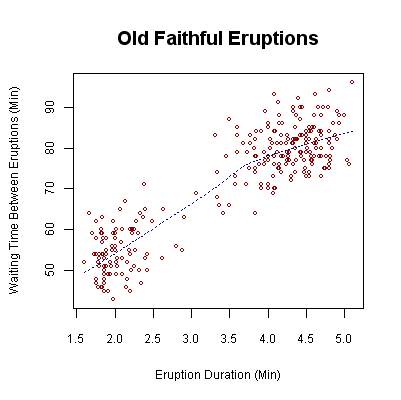
\includegraphics[width=1in,height=\textheight]{img/fig-1.png}
\caption{Plot 1: Plot eins}\label{fig:1}
\end{figure}

\begin{figure}
\centering
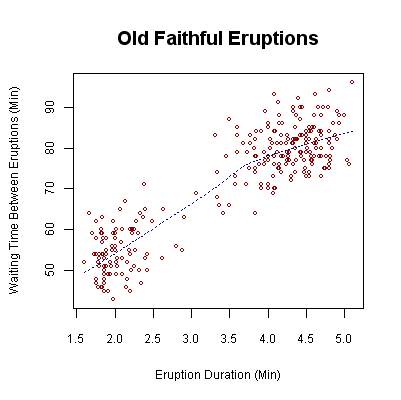
\includegraphics[width=1in,height=\textheight]{img/fig-1.png}
\caption{Plot 2: Plot zwei}\label{fig:2}
\end{figure}

Wir verweisen auf Plot \ref{fig:1} und Plots \ref{fig:1}, die
\ref{fig:2} mit Postfix \& fehlenden \ref{fig:3}.
